% Arlington County Board Structure and Performance study.
%
% Figures are NOT defined in this file. They are built from raw/ by run.sh and
% written to ../figures/pdf/, which \graphicspath points at below. To change a
% figure, edit its script in analysis/ and re-run. Never paste plot data here:
% that makes a second copy of the numbers, free to go stale.
\documentclass{article}

\usepackage{graphicx}
\usepackage{booktabs}
\usepackage[margin=1in]{geometry}
\usepackage{hyperref}

% Chicago notes-bibliography: a superscript number in the sentence, the full
% citation in a footnote, and the bibliography at the end. Chosen over
% author-date because this project's sources need caveats stated where the
% claim is - that O'Leary infers party affiliation, that Hjerpe's work is
% unpublished - and a footnote is the only place those fit.
%
% sources.bib is the registry the data shares: the `source` columns in
% data/clean/ hold citekeys from it, and bash run.sh refuses to build if one
% of them names an entry that is not here.
\usepackage[notes, backend=biber]{biblatex-chicago}
\addbibresource{sources.bib}

% The paper includes the PDF versions; figures/png/ is for slides and email.
\graphicspath{{../figures/pdf/}}

\title{Report for Arlington County Board}
\author{Sally Hudson and Alex Keena}
\date{September 2026}

\begin{document}

\maketitle

\section{Introduction}

\begin{figure}[htbp]
  \centering
  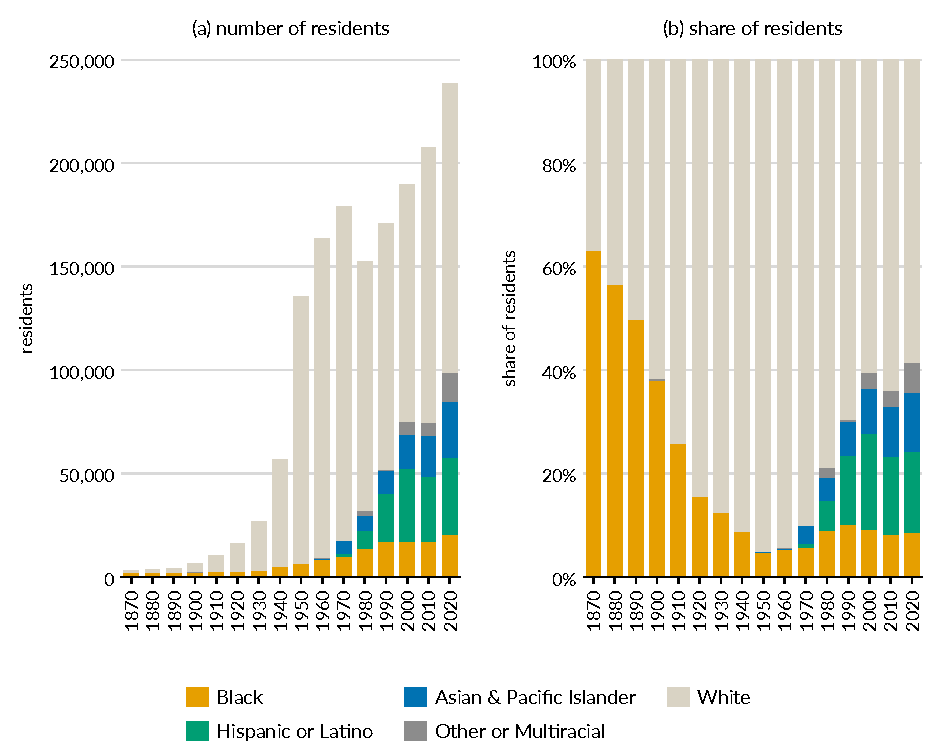
\includegraphics[width=\textwidth]{residents_by_race.pdf}
  \caption{Arlington County residents by race and ethnicity, 1870--2020.
  Panel (a) gives counts as reported; panel (b) gives each group's share.
  Hispanic/Latino and Asian American/Pacific Islander residents were not
  separately tabulated before 1970 and 1950 respectively, and are shown as zero
  before those years. The four categories sum to slightly more than the reported
  total in 1970 and 1990: panel (a) plots them as reported, so those bars sit
  above the total, while panel (b) rescales those columns to 100\%.}
  \label{fig:residents-race}
\end{figure}

\begin{figure}[htbp]
  \centering
  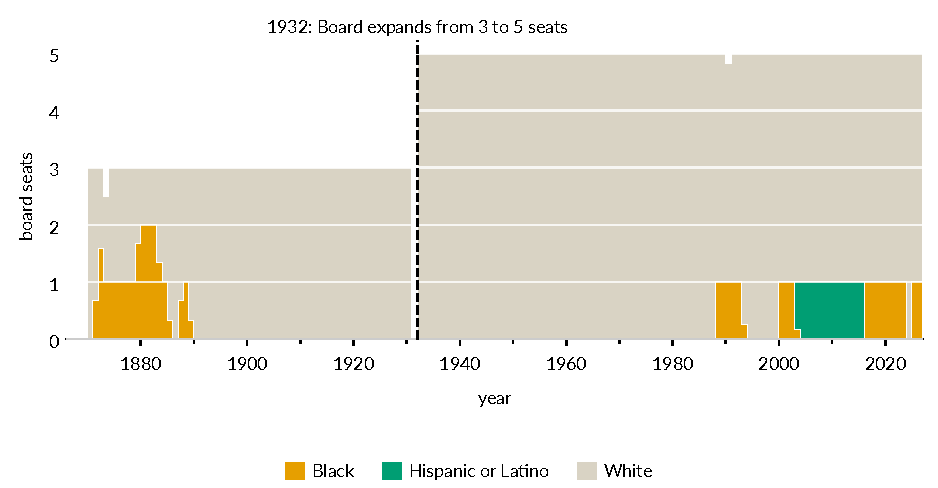
\includegraphics[width=\textwidth]{board_race.pdf}
  \caption{Composition of the Arlington County Board by race and ethnicity,
  1871--2026, in seats rather than shares. The dashed line marks 1932, when the
  Board expanded from three to five seats and magisterial districts were
  replaced by at-large elections. Half seats occur when a Board member resigned
  or died before the end of the year and was subsequently replaced. 1931 is not
  reported in the source data and appears as a gap. No Asian American or Pacific
  Islander member has served in any year, so no such category is drawn.}
  \label{fig:board-race}
\end{figure}

% Dormant until the first citation is written. biblatex lists only what is
% cited, so uncommenting this now prints an empty heading. To start citing:
% write \autocite[6]{oleary2010} in a sentence - the key comes from
% sources.bib, which is the same registry the data/clean/ source columns use -
% then uncomment the line below.
% \printbibliography[title={Works cited}]

\end{document}
